\section{Testing and Experiment}

This section discusses the testing scheme done in order to make sure the system
has met all feature requirements and it's working as intended. This secion also
further discusses the experimentation done on the system.

\subsection{Testing Scheme}

For the testing, four aspects will be tested. The four aspects are application,
data, end-to-end auto mode, and end-to-end override mode. The test cases for each
aspects can be seen in table \ref{tab-test-cases}.

\begin{table*}
      \caption{Test cases for each aspects}
      \centering
      \begin{tabular}{|c|p{10cm}|}
            \hline
            \textbf{Aspect}          & \textbf{Test cases}
            \\
            \hline
            Sensor                   & \begin{itemize}[leftmargin=*]
                                             \item measure the accuracy of MQ135 CO$_2$ ppm
                                                   reading,
                                             \item measure the accuracy of DHT22 temperature
                                                   reading, and
                                             \item measure the offset needed to turn servo
                                                   0\textdegree, 45\textdegree, or
                                                   90\textdegree.
                                       \end{itemize}
            \\
            \hline
            Application              & \begin{itemize}[leftmargin=*]
                                             \item app can show the newest
                                                   temperature and CO$_2$ data,
                                             \item app can show minimum, maximum, and
                                                   mean of the last 30 seconds of
                                                   temperature and CO$_2$ ppm and update it
                                                   automatically every 15 seconds,
                                             \item app can open and close door/window,
                                             \item app can change mode (auto to
                                                   override and the vice versa),
                                             \item app can show the last 12 hours of
                                                   notifications/alerts, and
                                             \item app can send email for alerts.
                                       \end{itemize}
            \\
            \hline
            Data                     & \begin{itemize}[leftmargin=*]
                                             \item Sensor data is saved to database
                                                   every 1 second, and
                                             \item PySpark script publishes mean,
                                                   minimum, and maximum statistics of the
                                                   last 30 seconds every 15 seconds to
                                                   Kafka.
                                       \end{itemize}
            \\
            \hline
            End-to-end auto mode     & \begin{itemize}[leftmargin=*]
                                             \item In normal condition (good air
                                                   quality), servo is 90\textdegree
                                                   (window/door is open),
                                             \item In high CO$_2$ condition,
                                                   servo is 0\textdegree
                                                   (window/door is closed), and
                                             \item In a situation where
                                                   humidity or temperature is high,
                                                   servo is 90\textdegree
                                                   (window/door is open).
                                       \end{itemize}
            \\
            \hline
            End-to-end override mode & \begin{itemize}[leftmargin=*]
                                             \item In normal condition (good air
                                                   quality) and servo is 0\textdegree
                                                   (window/door is closed), an
                                                   alert should be sent every 30
                                                   minutes,
                                             \item In high CO$_2$ condition and
                                                   servo is 90\textdegree (window/door
                                                   is open), an alert should be sent
                                                   every 30 minutes, and
                                             \item In a situation where
                                                   humidity or temperature is
                                                   high and servo is
                                                   0\textdegree (window/door is
                                                   closed), an alert should be
                                                   sent every 30 minutes
                                                   (window/door is open).
                                       \end{itemize}
            \\
            \hline
      \end{tabular}
      \label{tab-test-cases}
\end{table*}

\subsection{Experimental Setup}
In this section, we will describe the experimental setup of the proposed system.
There are two main spaces, which are a closed room and the outside of the room.
These two spaces are partitioned by a door and/or a window. Inside the room,
DHT22 sensor is placed to measure the temperature and humidity of the room.
Outside the room, MQ135 sensor is placed to measure the CO$_2$ ppm outside the room.
A servo motor is placed to open and close the door/window.
Experimental setup of the system can be seen in figure \ref{setup}.

\begin{figure}
      \centerline{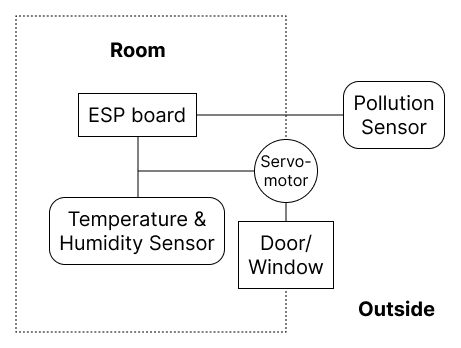
\includegraphics[scale=0.4]{resources/setup.png}}
      \caption{Experimental setup of the smart room air conditioner}
      \label{setup}
\end{figure}

Control setup of the system is when the door is open and all sensors are
indicating normal values or within an acceptable range. This system is will be
tested in the following scenarios:
\begin{enumerate}
      \item Using auto mode, a match will be lit and placed near the MQ135 sensor
            in order to increase the CO$_2$ ppm outside the room. The door should
            be closed to prevent bad air from coming in.
      \item Using auto mode, a match will be lit and placed near the DHT22 sensor
            to increase the temperature/humidity inside the room. The door should
            should be opened to let fresh air in.
      \item Using override mode, a match will be lit and placed near the MQ135
            sensor in order to increase the CO$_2$ ppm outside the room. If the door
            is opened, an email will be sent to warn the user to close the door.
      \item Using override mode, a match will be lit and placed near the DHT22
            sensor to increase the temperature/humidity inside the room. If the door
            is closed, an email will be sent to warn the user to open the door.
\end{enumerate}
